\subsection{Komponenten}
Bei den Komponenten musste darauf geachtet werden, dass diese den \"ausseren Einfl\"usse sowie den spezifischen Softwaretechnischen Daten genügen. Die einzelnen Geräte der Arbeit bestehen aus Rechnereinheit, Messsensor, WIFI-Adapter, Gehäuse sowie einer Spannungsversorgung.
\subsubsection{Rechnereinheit}
An die Rechnereinheit wurden sehr grosse Anforderungen gestellt, da diese bei $-40^\circ\text{C}$ aber auch bei über $40^\circ\text{C}$ die Auswertung durchf\"uhren muss. Ebenso muss die Rechnereinheitser viel Auswertung direkt durchführen, um sowenig wie m\"oglich direkt zu speichern. Der Rechnerkern des Gerätes besteht aus einem Allwinner H3, welcher einen Quad-core Cortex-A7 mit bis zu 1.2GHz Taktrate besitzt. Dieser Rechnerkern ist einer der am besten geeignetsten für das Gerät da auf diesem mehrere Prozesse gleichzeitig ablaufen können, dies ist nötig um die gew\"unschte Verarbeitungsgeschwindigkeit zu erreichen. Im Zuge dessen wurde ein vorgefertigtes Board in dem Gerät eingesetzt. Das eingesetzte Board ist ein NanoPi NEO von FriendlyARM. Der NanoPi NEO hat den oben genannten Quad-core Prozessor mitwelchem die Aufgabe gel\"ost werden kann. \\
Dieses Board bietet ebenso den Vorteil dass alles auf einer Fl\"ache von 40x40cm sich befindet. So kann das gesamte Ger\"at sehr kompakt gestaltet werden. Das Board wird mit einer externen Speicherkarte verwendet, auf welcher das Betriebssystem, in Falle von Fast and Curious, ist es Ubuntu 16.04 (Long Time Supported), sich befindet. \\
Nachteil an dem NanoPi NEO sind zum einen die eher schlechte Dokumentation sowie jede glich das Vorhandensein eines einzelnen USB Anschlusses. Aus diesem Grunde musste bei dem Ger\"at ein USB Dongle verwendet werden um den Messsensor sowie den USB-WIFI-Adapter anzuschliessen.

\begin{figure}[H]
  \centering
  \includegraphics[height=0.6\textwidth]{Hardware/NanoPi_Neo.jpg} 
  \caption{Layout des NanoPi NEO.}
  \label{bArchitektur}
\end{figure}

\subsubsection{Messsensor}
Der Messsensor des Ger\"ates muss in der Lage sein  Daten der Verkehrsteilenehmer zu liefern, mit denen dann die weitere Auswertung geschehen kann. Es müssen aus den Daten des Messsensors Kenngr\"ossen extrahiert werden welche die Verkehrsteilnehmer eindeutig identifizieren lässt. Es wurde auf eine Kamera zurückgegriffen, welche im Stande ist zwei Fahrspuren zu überdecken und mindestens drei Bilder pro vorbeifahrendem Verkehrsteilnehmer aufzunehmen. \\
Mithilfe folgender Berechnung wurde die geeignete Kamera sowie das passende Objektiv dazu gefunden.
\begin{citemize}

\item Kamera mit 30 FPS \\
$l_{ 1,30 } = \frac{ 22.22 m/s }{ 30 FPS} = 0.75 m$ \\ 
$l_{ 4,30 } = 4 * l_{1,30} = 3 m$\\
$\alpha_{30} = 2* \arctan(l_{4,30 }) \approx 150^\circ$ \\\\


\item Kamera mit 60 FPS \\
$l_{ 1,60 } = \frac{ 22.22 m/s }{ 60 FPS} = 0.37 m$ \\ 
$l_{ 4,60 } = 4 * l_{1,30} \approx 1.5 m$\\
$\alpha_{60} = 2* \arctan(l_{4,60 }) \approx 120^\circ$ \\\\
\end{citemize}

\begin{figure}[H]
  \centering
  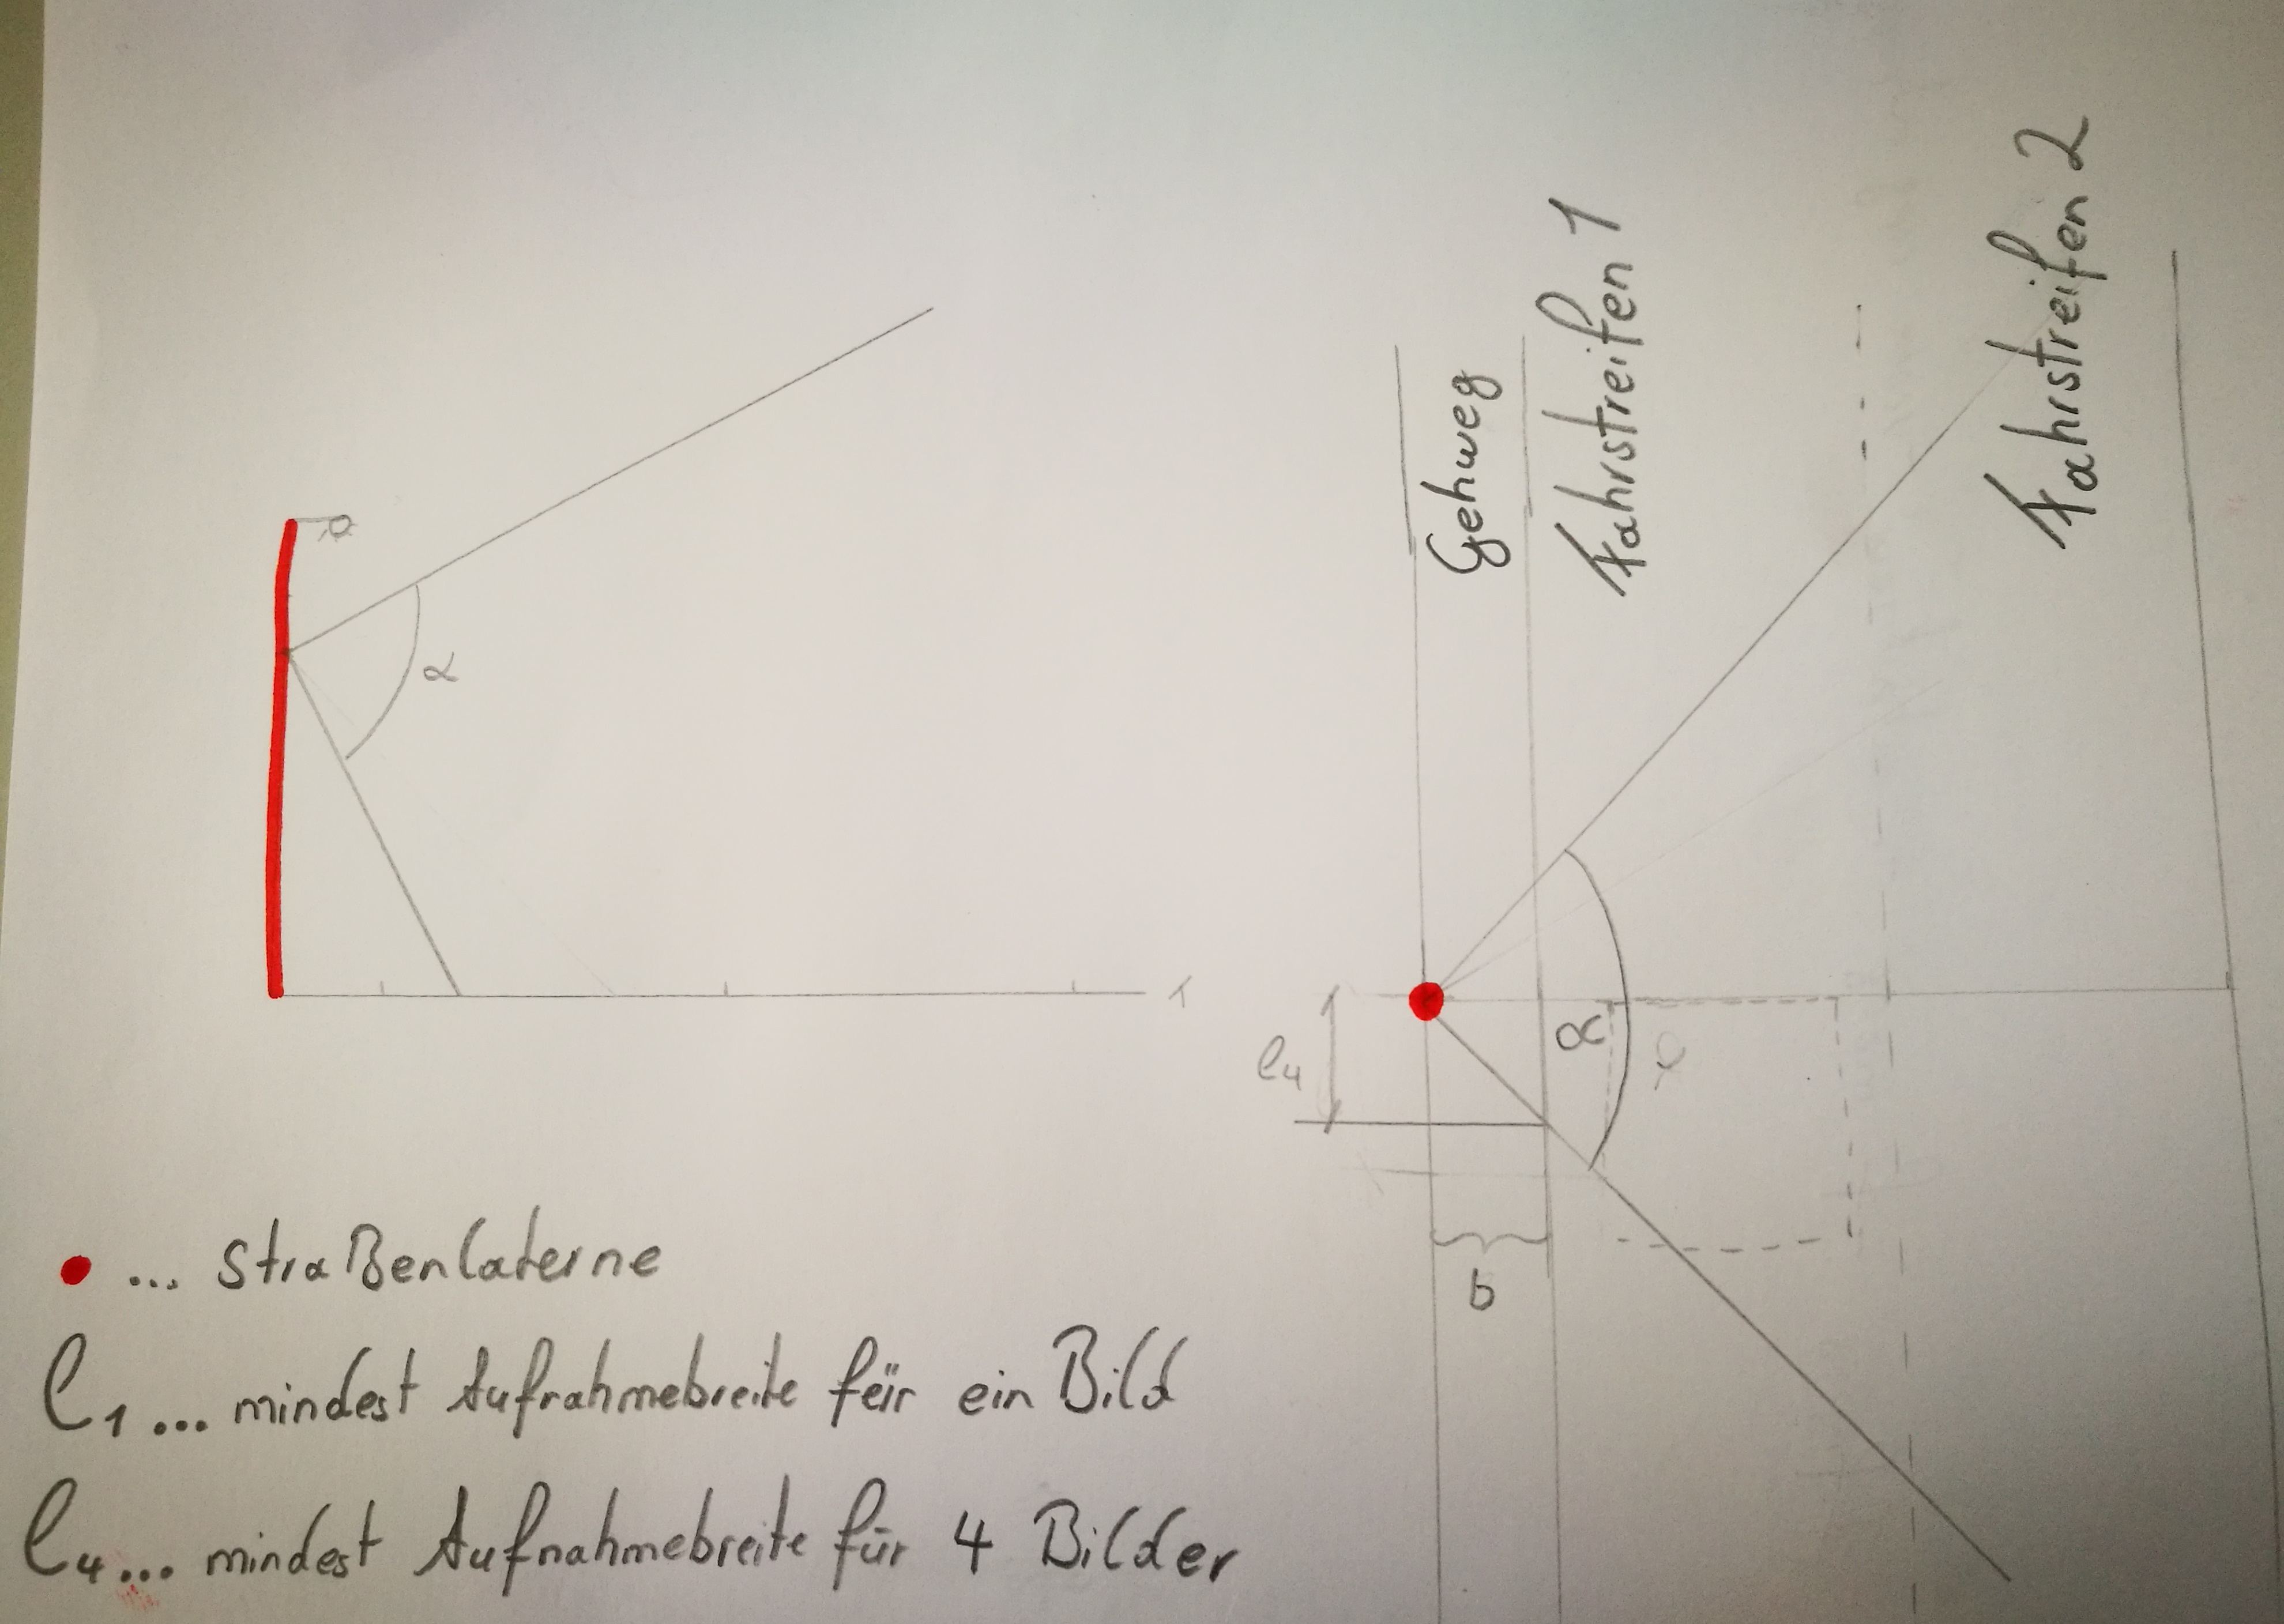
\includegraphics[height=0.49\textwidth]{Hardware/ObjektivBerechnung.jpg} 
  \caption{Skizze zur Berechnung der Kamera Daten.}
  \label{bArchitektur}
\end{figure}

Durch diese Berechnung wurde auf eine Kamera eingesetzt, welche mit einer Framerate Anzahl von 60FPS Bilder aufnimmt. \\
In dem produzierten Prototypen wurde eine ELP 1080p Full HD H.264 Kamera mit 3.6mm Objektiv verwendet. 
Diese Kamera hat den Vorteil, dass die gewünschten Treiber auf dem Betriebssystem schon installiert sind und die Kamera sehr Preisgünstig zu haben ist. Diese Kamera besitzt bei einer FPS Anzahl von 60 eine Auflösung von 640x480 Pixel und einem 3.6mm Objektiv. Diese Anzahl an Pixel reicht aus um die nötigen Daten der Verkehrsteilnehmer zu extrahieren.

\subsubsection{WIFI-Adapter}
Um das Ger\"at Steuern und \"Uberwachen zu können wird eine kabellose Verbindung benötigt. Dies ist am einfachsten über eine WIFI-Verbindung zu erm\"oglichen. Da das NanoPi NEO keine internen Funksender eingebaut hat wird ein WIFI-Adapter ben\"otigt. Dazu kann jeder WIFI-Adapter verwendet werden, welche f\"u Linux Systeme Treiber Supporten. Werden f\"ur die Ger\"ate unterschiedliche WIFI-Adapter eingesetzt, so muss nach der Anleitung f\"ur die Installation der Ger\"ate vorgegangen werden, und die Namen der Adapter ge\"andert werden.\\
Die einzige Anforderung an den WIFI-Adapter ist es dass dieser \"uber USB angeschlossen wird. Die Ger\"ate welche produziert wurden haben unterschiedliche WIFI-Adapter eingebaut und es funktioniert mit allen WIFI-Adaptern ohne irgendwelche Probleme. (Verbindung geschieht über einen Hotspot vom Endgerät zu NanoPi NEO)

\subsubsection{Spannungsversorgung}
Die Spannungsversorgung der Ger\"ate wurde mittels Autobatterie und Spannungswandler realisiert. Das gesamte Ger\"at ben\"otigt bei Volllast ca. 400mA Strom. Die verwendeten Autobatterien haben eine Kapazit\"at von 44Ah und eine Spannung von 12V. \\

$\frac { 44000\quad mAh\quad \times \quad 12\quad V }{ 400\quad mAh\quad \times \quad 5\quad V } =\quad 264\quad h=\quad 11d$ \\

Wie aus dieser Berechnung entnommen werden kann bel\"auft sich die Betriebszeit mit einer Akku Ladung theoretisch auf ca. 11 Tage. Wie erwartet ist die tats\"achliche Laufeit der Ger\"ate kleiner als die Berechnete, jedoch betr\"agt die tats\"achliche Laufzeit etwa di h\"alfte von ca. 5 Tagen. \\
In einer Tast\"achlichen Fertigung der Ger\"ate muss eine neue Spannungsquelle gefunden werden da Autobatterien beinahe immer Bleihaltig sind. Es können Lithium Ionen Akkus verwendet werden, jedoch waren diese f\"ur die Prototypen zu teuer und nicht rentabel. 

\subsubsection{Gehäuse}
Das Geh\"ause der Prototypen besteht aus einer Kunstoffbox, in welcher fr\"uher Lebensmittel sich befande. In diesem Geh\"ause wurden alle Komponenten welche oben genannt wurden, mittels Klettverschluss angebracht um die Komponenten ohne Geh\"ause weiter zu verwenden. Dies erm\"oglichte eine leichtere Bedienung bei der programmierung der Software. An dem Geh\"ause wurden zwei Gewindestangen angebracht um die Ausrichtung des Ger\"ates einstellen zu k\"onnen. Desweiteren wurde in den Deckel der Kunstoffboxen Schlitze geschnitten, um die Abw\"arme der Komponenten besser nach aussen zu bef\"ordern. Die Geh\"ause werden an den Strassenlaternen mittels grossen Kabelbindern befestigt.\\
\textbf{Wichtig: In den Geh\"ausen befindet sich keine Batterie.}\\
Aus Sicherheitsgr\"unden wurde ein zweipoliges Kabel von den Ger\"aten nach unten geogen und an den Polen der Batterie befestigt. 

\begin{figure}[H]
  \centering
  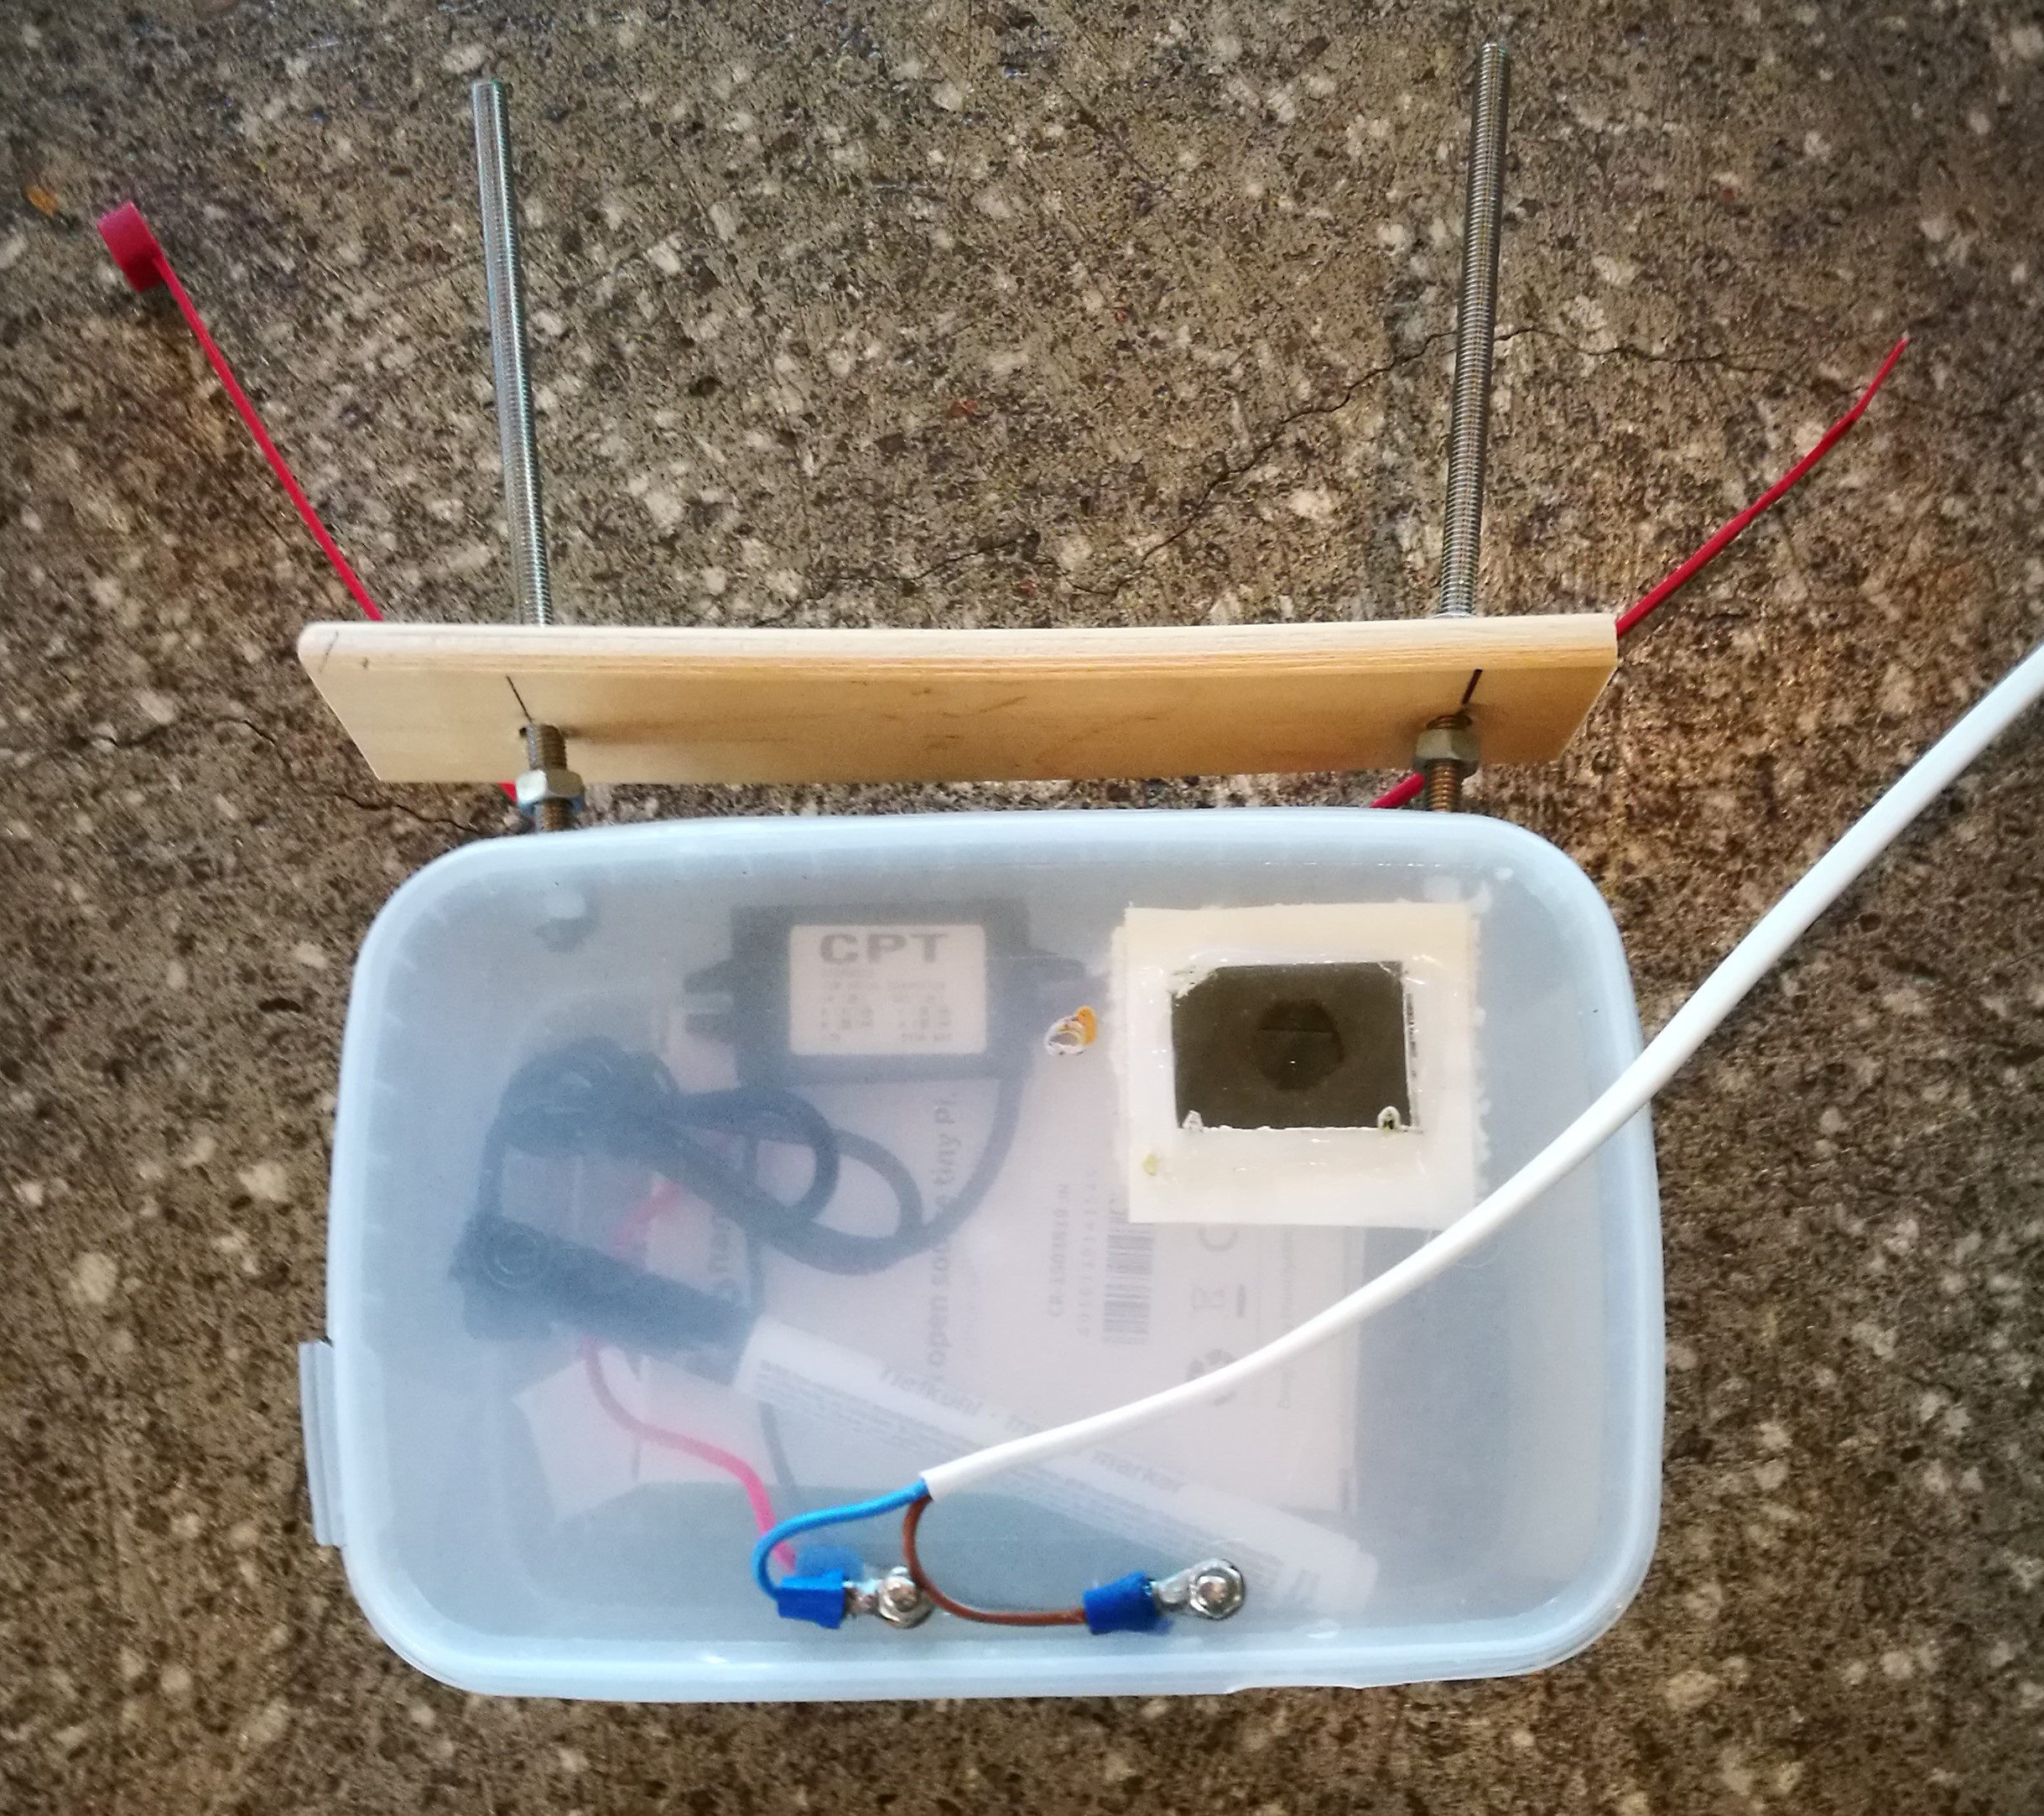
\includegraphics[height=0.49\textwidth]{Hardware/Gehaeuse.jpg} 
  \caption{Foto eines leeren Geh\"auses.}
  \label{bArchitektur}
\end{figure}
